42. Перед вами МНОГОУГОЛЬНИК. У него может быть сколько угодно ВЕРШИН. ({\it На предложенном рисунке их всего 6, для примера.}) Представьте себе тридцатиугольник (у него 30 вершин). Одну из его вершин соединим отрезками со всеми остальными. На сколько треугольников мы разделим тридцатиугольник?
\begin{center}
\begin{figure}[ht!]
\center{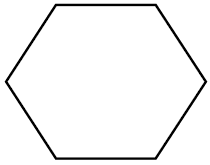
\includegraphics[scale=0.35]{6.png}}
\end{figure}
\end{center}

ewpage

oindent43. В клетках квадрата $3\times3$ были записаны натуральные числа так, что суммы в каждой строке, в каждом столбце и на каждой диагонали были одинаковыми. Некоторые числа стёрли. Восстановите стёртые числа.
\begin{center}
\begin{figure}[ht!]
\center{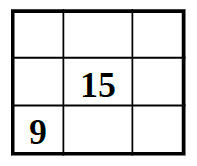
\includegraphics[scale=0.35]{7.png}}
\end{figure}
\end{center}
